\section{Theorie}
\label{sec:Theorie}

Seit einigen Jahren findet Mikrowellen-Strahlung in vielen Bereichen eine Anwendung. 
Den meisten Leuten fällt beim Begriff Mikrowelle vermutlich als erstes der Mirkowellen-Ofen ein,
da dieses Gerät ein wichtiger Bestandteil vieler Küchen heutzutage ist.
Aber Mikrowellen haben noch deutlich mehr Anwendungsgebiete:
\begin{itemize}
    \item jegliche Art der kabellosen Kommunikation. (Mobilfunk, WLAN, Bluetooth,...)
    \item Radartechnik
    \item Navigation über GPS
    \item Radio astronomy
    \item Spektroskopie
    \item ...
\end{itemize}

Das Wort \enquote{Mikrowellen} ist allerdings irreführend, da die Wellenlänge von elektromagnetische Strahlung in der Größenordnung Mikrometer 
Infrarot-Strahlung ist.
Mikrowellen-Strahlung liegt hingegen im Wellenlängenbereich von Millimeter bis Meter bzw. einem Frequenzbereich von $\SI{300}{\mega\hertz}$ bis $\SI{300}{\giga\hertz}$.
Und die \enquote{Mikro} in Mikrowellen steht eher für klein als für die Größenordnung.

\subsection{Erzeugung von Mikrowellen mittels eines Reflexklystrons}
\label{ssec:Erzeugung}

Um Mikrowellen-Strahlung mit einer hohen Intensität erzeugen zu können, hat man ein sogenanntes Klystron entwickelt um hochfrequente Signale verstärken zu können.
Da diese Klystrons allerdings groß sind, wurden sie zum sogenannten Reflexklystron weiterentwickelt.
Die Funktionsweise des Reflexklystrons ist sehr ähnlich zum Klystron und lässt sich besser am Klystron erklären.
Beide Geräte sind in \autoref{fig:wiki_klystron} schematisch dargestellt.

\begin{figure}
    \centering
    \begin{subfigure}{0.45\textwidth}
        \centering
        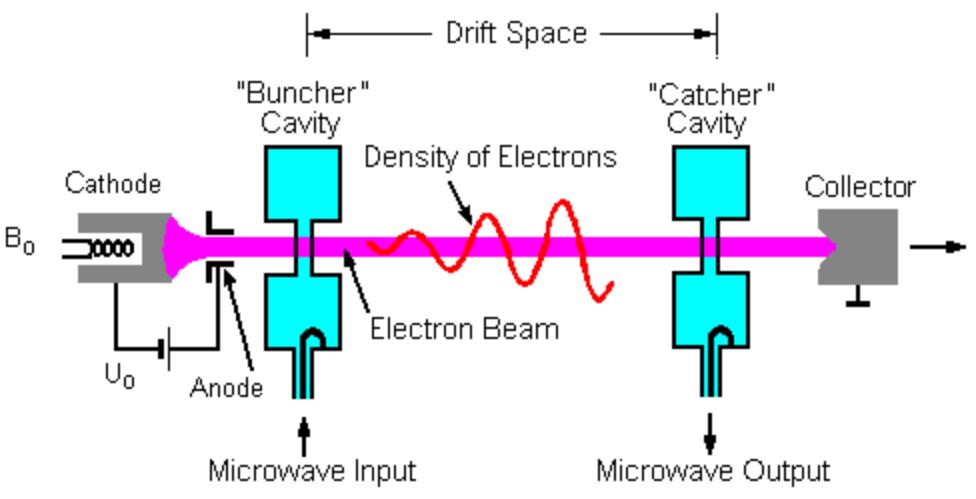
\includegraphics[width=\textwidth]{images/klystron.png}
        \caption{Klystron}
        \label{fig:klystron}
    \end{subfigure}
    \begin{subfigure}{0.45\textwidth}
        \centering
        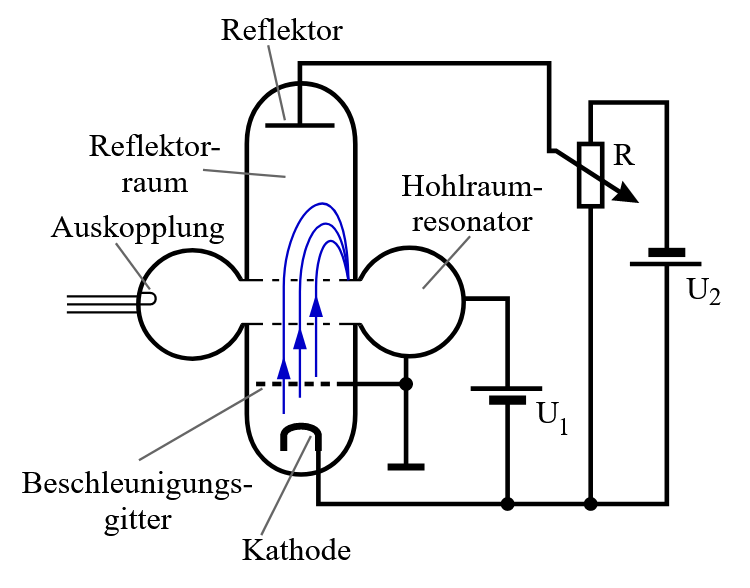
\includegraphics[width=\textwidth]{images/reflexklystron.png}
        \caption{Reflexklystron}
        \label{fig:reflexklystron}
    \end{subfigure}
    \caption{Schematische Skizzen vom Klystron und Reflexklystron \cite{wiki_klystron}}
    \label{fig:wiki_klystron}
\end{figure}

Elektronen werden von einer Glühkathode aus beschleunigt. 
Diese treten dann in einen \enquote{Buncher} Hohlraum ein.
In diesem Hohlraum schwingt ein elektrisches, annähernd homogenes Feld in Parallel zur Bewegungsrichtung der Elektronen.
Diese Schwingung wird durch ein Eingangssignal angeregt und der Hohlraum funktioniert auf dem Prinzip eines RC-Schwingkreises,
wobei in der Mitte ein Kondensator und außen eine Art Spule mit einer Windung ist.
Durch das schwingende elektrische Feld werden die Elektronen unterschiedlich stark beschleunigt oder abgebremst (Geschwindigkeitsmodulation)
und es entstehen auf dem Weg zum nächsten Hohlraum \enquote{Bunches}, also Häufungen von Elektronen. (Dichtemodulation)

In dem \equote{Catcher} Hohlraum sollten die Elektronbunches genau so ankommen, dass sie die Resonanzfrequenz des Hohlraums treffen und dort die Schwingung anregen.
Da allerdings hier die Elektronen sehr stark abgebremst werden, wird viel Energie in die angeregte Schwingung abgegeben 
und das so erzeugte Ausgangssignal hat eine deutlich höher Intensität als das Eingangssignal.

Beim Reflexklystron erfüllt ein Hohlraum beide soeben beschriebenen Funktionen und die Elektronen werden durch einen Reflektor in den gleichen Hohlraum zurückgeleitet.
Die so entstandene Schwingung kann z.B. über einen Draht oder einen Hohlleiter ausgekoppelt werden.

Da die Elektronen zum richtigen Zeitpunkt und in Bunches auf dem Rückweg wieder im Hohlraum ankommen müssen, 
müssen die Beschleunigungsspannung, die Reflektorspannung und die Abmessungen des Hohlraums
so angepasst werden, dass eine maximale Ausgangsleistung erreicht wird.
Eine optimale Flugdauer der Elektronen ist 
\begin{equation}
    \tau = T_0 (n+3/4) \, ,
\end{equation}
wobei $T_0$ die Resonanzfrequenz des Hohlraums ist und $n$ eine natürliche Zahl (oder 0) ist und eine Mode kennzeichnet.
Wie sich Amplitude und Frequenz des Ausgangssignals durch die Reflektorspannung verändert ist in \autoref{fig:modulation} zu sehen.

\begin{figure}
    \centering
    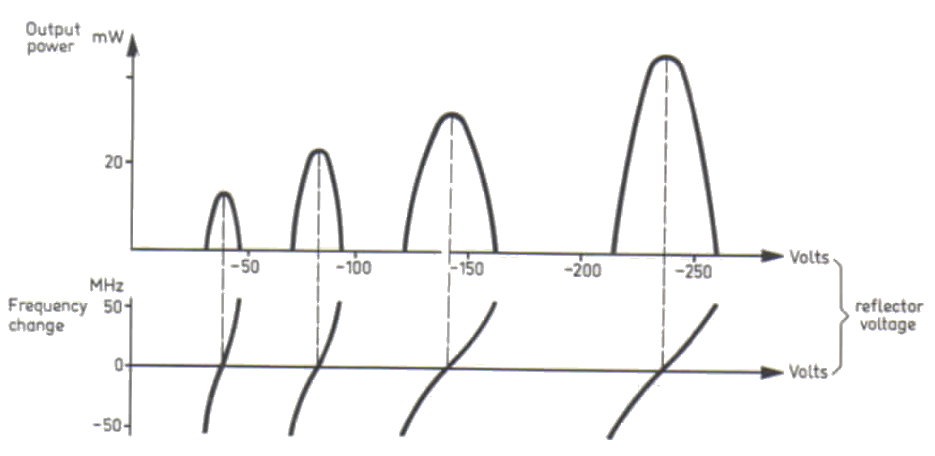
\includegraphics[width=0.7\textwidth]{images/modulation_white.png}
    \caption{Amplituden- und Frequenzmodulation des Reflexklystrons in Abhängigkeit der Reflektorspannung \cite{V53_old}}
    \label{fig:modulation}
\end{figure}

\subsection{Mikrowellen auf Hohlleitern}
\label{ssec:Hohlleiter}

